
This chapter describes the methodology followed in the development of this thesis.
This chapter comprises the following sections: Section \ref{sec:ch3-tools} describes the computational tools utilized in this work, Section \ref{sec:ch3-math} presents Moltres' mathematical basis, Section \ref{sec:ch3-bench} outlines the organization of the OECD/NEA MHTGR-350 Benchmark, and Section \ref{sec:ch3-mhtgr} summarizes the characteristics of the MHTGR-350.

\section{Computational tools}
\label{sec:ch3-tools}

The following sections describe the computational tools that participated in the development of this thesis.
The main computational tool was Moltres \cite{lindsay_introduction_2018}, described in Section \ref{sec:ch3-moltres}.
However, a description of Moltres is incomplete if not accompanied by an introduction to the underlying framework MOOSE \cite{gaston_moose_2009}, presented in Section \ref{sec:ch3-moose}.
Additionally, Chapter \ref{ch:neutronics} uses Serpent \cite{leppanen_development_2007}\cite{leppanen_calculation_2014} for obtaining group constants that serve as an input to Moltres. Section \ref{sec:ch3-serpent} summarizes Serpent's most important features.

\subsection{MOOSE}
\label{sec:ch3-moose}

% intro
MOOSE is a computational framework that supports engineering analysis applications.
In a nuclear reactor, several partial differential equations describe the physical behavior.
These equations are typically nonlinear, and they are often strongly coupled to each other.
\gls{MOOSE} targets such systems and solves them in a fully coupled manner.

% more details about MOOSE
\gls{MOOSE} is an open-source FEM framework under a \gls{LGPL}.
The framework itself relies on LibMesh \cite{kirk_libmesh_2006}, an LGPL finite element library, and PetSc, a \gls{BSD}-licensed toolkit for solving nonlinear equations \cite{balay_petsc_2016}.
MOOSE applications define weak forms of the governing equations and modularize the physics expressions into "Kernels."
Kernels are C++ classes containing methods for computing the residual and Jacobian contributions of individual pieces of the governing equations.
\gls{MOOSE} and LibMesh translate them into residual and Jacobian functions.
These functions become inputs into PetSc solution routines.

\gls{MOOSE} utilizes the \gls{JFNK} method \cite{knoll_jacobian-free_2004} mathematical structure \cite{gaston_moose_2009}.
\gls{JFNK} methods are synergistic combinations of Newton-type methods for superlinearly convergence of nonlinear equations and Krylov subspace methods for solving the Newton correction equations.
The Jacobian-vector product links the two methods.
JFNK methods compute such products approximately without forming and storing the elements of the true Jacobian.
The ability to perform a Newton iteration without forming the Jacobian gives JFNK methods potential for application throughout problems governed by nonlinear partial differential equations.

All the software built on the MOOSE framework shares the same \gls{API}.
The applications, by default, utilize monolithic and implicit methods \cite{lindsay_introduction_2018}.
This feature facilitates relatively easy coupling between different phenomena and allows for great flexibility, even with a great variance in time scales \cite{novak_pronghorn_2018}.
Additionally, the framework and its applications use \gls{MPI} for parallel communication and allow deployment on massively-parallel cluster-computing platforms.

\subsection{Moltres}
\label{sec:ch3-moltres}

\textit{Moltres} is a MOOSE-based application initially designed for modeling fluid-fuelled \glspl{MSR}.
Moltres inherits all the attributes from MOOSE as its application.
Moltres is an open-source simulation tool that operates under an LGPL.
It uses \textit{git} for version control, emphasizing its openness and promoting quality through peer review.
Moltres openness is an important feature and contrasts previous multi-physics applications, which operated under restrictive licenses.

Moltres solves arbitrary-group neutron diffusion, delayed neutron precursor concentration, and temperature governing equations.
It can solve the equations in a fully-coupled way or solve each system independently, allowing for great flexibility and making it applicable to a wide range of nuclear engineering problems.

Moltres is the primary tool in the development of this thesis.
Its role is to simulate prismatic HTGRs.
Chapter \ref{ch:neutronics} and \ref{ch:thermalfluids} compare the results calculated by Moltres and other software to validate Moltres' calculation scheme.
This work also intends to identify Moltres flaws in prismatic HTGR simulations and sets a basis for future work.

\subsection{Serpent}
\label{sec:ch3-serpent}

The Serpent Monte Carlo code \cite{leppanen_development_2007} \cite{leppanen_serpent_2015} is a three-dimensional continuous-energy neutron transport application developed by the VTT Technical Research Centre of Finland, and it has been in public distribution since 2009.
Monte Carlo neutron transport tools have several reactor physics applications related to criticality safety analyses, radiation shielding problems, detector modeling, and validation of deterministic solvers.
The Monte Carlo method's main advantage is its capability to model geometry and interaction physics without significant approximations.
The main disadvantage is that simulating complex systems is computing-intensive, restricting applications to some extent.

In general, Serpent serves two purposes: (1) reactor modeling and (2) group constant generation.
In reactor modeling, the Monte Carlo simulation itself represents the solution to the full-scale problem.
In group constant generation, the transport simulation produces input parameters for a deterministic solver.
Based on a few energy groups, deterministic solvers allow for carrying out coupled full-core analyses.

In this work, Serpent produces group constants that serve as an input for Moltres and solves for neutron fluxes in high geometric fidelity and continuous energy cross-sections.
This last step provides the reference solutions for the validation of the Moltres calculation scheme.
This work used Serpent 2.1.31 and the cross-section library JEFF3.1.2 for the calculations.
The reason for using Serpent to generate group constants is due to its ability to run explicit simulations of randomly located TRISO particles.
Applying a simple volume homogenization proves inaccurate due to the resonance self-shielding effect of the kernel and coated layers \cite{strydom_results_2015}.
Although the particles' explicit modeling is time-consuming, costly, and impractical for most applications, it is necessary.

\section{Mathematical basis}
\label{sec:ch3-math}

The last section introduced Moltres as the primary computational tool utilized in this thesis.
This section presents this thesis' mathematical basis, which are the equations that describe the neutronics and thermal-fluids of prismatic HTGRs in the steady-state limit.
For a more detailed explanation, refer to Section \ref{appendix:equations}.
Moltres and MOOSE heat conduction module translate these equations into kernels.

\subsection{Diffusion and precursors equations}

% Neutronics
Moltres translates the multi-group diffusion equations into kernels, equations that describe the steady-state behavior of the neutron flux and calculates the multiplication factor \cite{duderstadt_nuclear_1976}

\begin{align}
  % diffusion-eigenvalue calculation
  \nabla \cdot D_g \nabla \phi_g - \Sigma_g^r \phi_g & + \sum_{g' \ne g}^G \Sigma_{g'\rightarrow g}^s \phi_{g'} +
  \chi_g^t \sum_{g' = 1}^G \frac{1}{k_{eff}}\nu \Sigma_{g'}^f \phi_{g'} = 0 \label{eq:diffusion-eig}
  \intertext{where}
  & D_g = \mbox{group $g$ diffusion coefficient } [cm] \notag \\
  & \phi_g = \mbox{group $g$ neutron flux } [n \cdot cm^{-2} \cdot s^{-1}] \notag \\
  & \Sigma_g^r = \mbox{group $g$ macroscopic removal cross-section } [cm^{-1}] \notag \\
  & \Sigma_{g'\rightarrow g}^s = \mbox{group $g'$ to group $g$ macroscopic scattering cross-section } [cm^{-1}] \notag \\
  & \chi_t^p = \mbox{group $g$ total fission spectrum } [-] \notag\\
  & G = \mbox{number of discrete energy groups } [-] \notag \\
  & k_{eff} = \mbox{multiplication factor } [-] \notag \\
  & \nu = \mbox{number of neutrons produced per fission } [-] \notag \\
  & \Sigma_g^f = \mbox{group $g$ macroscopic fission cross-section } [cm^{-1}]. \notag
\end{align}

% Boundary conditions
In different sections of this thesis, Moltres simulations apply several boundary conditions.
The vacuum boundary condition \cite{duderstadt_nuclear_1976} states that no neutrons penetrate the boundary in the inward direction --- the incoming current density is equal to zero
\begin{align}
   & J^-_g(r_s) = \frac{1}{4} \phi_g(r_s) + \frac{D}{2} \hat{n_s} \cdot \nabla \phi_g(r_s) = 0 \label{eq:vacuumbc} \\
   \intertext{where}
   & J^-_g(r) = \mbox{incoming current density } [n \cdot cm^{-2} \cdot s^{-1}] \notag \\
   & r_s = \mbox{position of the boundary } [cm] \notag \\
   & \hat{n_s} = \mbox{normal direction to the boundary } [-]. \notag
\end{align}

The reflective boundary condition states that no neutrons penetrate the boundary --- the current density is equal to zero 
\begin{align}
   & J_g(r_s) = 0 \label{eq:reflecbc}
   \intertext{where}
   & r_s = \mbox{position of the boundary } [cm] \notag \\
   & J_g(r) = \mbox{current density } [n \cdot cm^{-2} \cdot s^{-1}]. \notag
\end{align}

The periodic boundary condition states that the flux and current density are equal on both sides of the boundary
\begin{align}
   & \phi_g(r_{s^-}) = \phi_g(r_{s^+}) \label{eq:perbc1} \\
   & J_g(r_{s^-}) = J_g(r_{s^+}) \label{eq:perbc2}
   \intertext{where}
   & J_g(r) = \mbox{current density } [n \cdot cm^{-2} \cdot s^{-1}] \notag \\
   & r_{s^\pm} = \mbox{left and right side of $r_s$ boundary } [cm]. \notag
\end{align}

\subsection{Thermal-fluids}
\label{ch3:th}

The three-dimensional steady-state heat conduction equation solves the temperature in the fuel, helium gap, moderator, coolant film, and reflector \cite{melese_thermal_1984}

\begin{align}
  & k_i \nabla^2 T_i + Q_i = 0 \label{eq:tempsolid} \\
  \intertext{where}
  & i = \mbox{f (fuel), g (helium gap), m (moderator), cf (coolant film), r (reflector)} \notag \\
  & k_i = \mbox{material $i$ thermal conductivity  } [W \cdot cm^{-1} \cdot K^{-1}] \notag \\
  & T_i = \mbox{material $i$ temperature } [^{\circ}C] \notag \\
  & Q_i = \mbox{material $i$ volumetric heat source } [W \cdot cm^{-3}]. \notag
\end{align}

Equations \ref{eq:heatsource1} and \ref{eq:heatsource2} define the heat source in the stand-alone and coupled calculations, respectively

\begin{align}
  & Q_f = Q_0 \label{eq:heatsource1} \\
  & Q_f = \sum_{g = 1}^{G} \epsilon_g^f \Sigma_g^f \phi_g \label{eq:heatsource2} \\
  & Q_g = Q_m = Q_{cf} = Q_r = 0 \label{eq:heatsource3}
  \intertext{where}
  & Q_i = \mbox{material $i$ volumetric heat source } [W \cdot cm^{-3}] \notag \\
  & \epsilon_g^f = \mbox{energy released per fission } [J] \notag \\
  & \Sigma_g^f = \mbox{group $g$ macroscopic fission cross-section } [cm^{-1}] \notag \\
  & \phi_g = \mbox{group $g$ neutron flux } [n \cdot cm^{-2} \cdot s^{-1}]. \notag
\end{align}

% coolant
The governing equation of the coolant is the one-dimensional steady-state energy conservation equation \cite{white_viscous_2006}\cite{tak_practical_2012}

\begin{align}
 	& \rho_{c,i} u_i \frac{\partial}{\partial z} (c_{p,c} T_c) = q'''_{conv} 	\label{eq:tempcool} \\
  & q'''_{conv} = h\frac{\varepsilon}{A} (T_i-T_c) \label{eq:convection}
  \intertext{where}
  & \rho_{c, i} = \mbox{inlet coolant density } [kg \cdot cm^{-3}] \notag \\
  & u_i = \mbox{inlet coolant velocity } [cm \cdot s^{-1}] \notag \\
  & c_{p,c} = \mbox{coolant specific heat capacity } [J \cdot kg^{-1} \cdot K^{-1}] \notag \\
  & T_c = \mbox{coolant temperature } [^{\circ}C] \notag \\
  & q'''_{conv} = \mbox{convective heat transfer } [W \cdot cm^{-3}] \notag \\
  & A = \mbox{cross-sectional area } [cm^2] \notag \\
  & h = \mbox{heat transfer coefficient } [W \cdot cm^{-2} \cdot K^{-1}] \notag \\
  & T_i = \mbox{solid temperature } [^{\circ}C]. \notag
\end{align}

Equation \ref{eq:film-conduc} calculates the film thermal conductivity $k_f$ \cite{melese_thermal_1984}

\begin{align}
  & Nu = 0.023 Re^{0.8} Pr^{0.4} \label{eq:dittus} \\
  & h = \frac{Nu \cdot k_c}{D_h}  \\
  & k_f = h R_{cf} ln(R_{cf}/R_c) \label{eq:film-conduc}
  \intertext{where}
  & Nu = \mbox{Nusselt number } [-] \notag \\
  & Re = \mbox{Reynolds number } [-] \notag \\
  & Pr = \mbox{Prandtl number } [-] \notag \\
  & h = \mbox{heat transfer coefficient } [W \cdot cm^{-2} \cdot s^{-1}] \notag \\
  & D_h = \mbox{hydraulic diameter } [cm] \notag \\
  & k_c = \mbox{coolant thermal conductivity } [W \cdot cm^{-1} \cdot K^{-1}] \notag \\
  & k_{cf} = \mbox{coolant film thermal conductivity } [W \cdot cm^{-1} \cdot K^{-1}] \notag \\
  & R_{cf} = \mbox{coolant film radius } [cm] \notag \\
  & R_c = \mbox{coolant channel radius } [cm]. \notag
\end{align}

\section{OECD/NEA MHTGR-350 Benchmark}
\label{sec:ch3-bench}

Chapters \ref{ch:neutronics} and \ref{ch:thermalfluids} conduct several exercises of the benchmark \cite{oecd_nea_benchmark_2017} using Moltres.
The \gls{OECD}/\gls{NEA} defined such a benchmark using the \gls{MHTGR}-350 reactor \cite{silady_licensing_1988} as the reference design.
The scope of the benchmark is twofold: (1) establish a well-defined problem, based on a common given data set, to compare methods and tools in core simulation and thermal fluids analysis, and (2) test the depletion capabilities of various lattice physics tools available for prismatic HTGRs.
The benchmark defines several phases and exercises, summarized in Table \ref{tab:benchmark}.

\begin{table}[htbp!]
  \centering
  \caption{Description of the OECD/NEA MHTGR-350 Benchmark phases and exercises.}
  \begin{tabular}{lcl}
\toprule
Phase               & Exercise & Description                                             \\
\midrule
\multirow{3}{*}{I}  & 1        & Neutronics solution with fixed cross-sections           \\
                    & 2        & Thermal fluids solution with given heat sources         \\
                    & 3        & Coupled neutronics-thermal fluids steady state solution \\
\midrule
\multirow{4}{*}{II} & 1        & Depressurized Conduction Cooldown without reactor trip  \\
                    & 2        & Pressurized Conduction Cooldown with reactor trip       \\
                    & 3        & Water ingress with reactor trip                         \\
                    & 4        & Power 100-80-100 load follow                            \\
\midrule
III                 & -        & Lattice Depletion Calculation                           \\
\bottomrule
  \end{tabular}
  \label{tab:benchmark}
\end{table}

\section{MHTGR-350 Reactor Description}
\label{sec:ch3-mhtgr}

This section describes the \gls{MHTGR}-350 reactor.
The core consists of an array of hexagonal fuel elements in a cylindrical arrangement, pictured in Figure \ref{fig:layout}.
Nineteen graphite replaceable reflector elements compose the inner reflector region.
A ring of identically sized graphite replaceable reflector elements surrounds the fuel elements.
Then, a region of permanent reflector elements surrounds the replaceable reflectors.
The reactor vessel encases all the elements.
Ten layers of fuel elements stacked on top of each other compose the 66 fuel columns that integrate the active core.
Figure \ref{fig:layoutb} shows an axial view of the reactor.
Table \ref{tab:maincharac} summarizes the reactor's main characteristics.

\begin{figure}[htbp!]
    \centering
    \subfloat[Core radial layout. Image reproduced from \cite{oecd_nea_benchmark_2017}.]{
        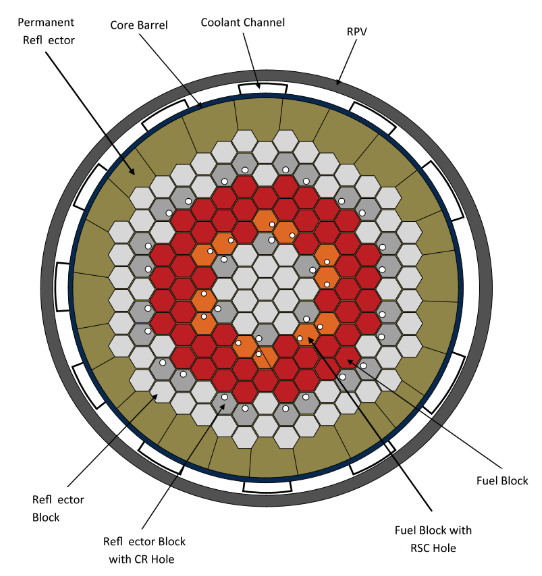
\includegraphics[width=0.45\textwidth]{figures/radial-layout.png}
    }
    \subfloat[Core axial layout. Image reproduced from \cite{oecd_nea_benchmark_2017}.\label{fig:layoutb}]{
        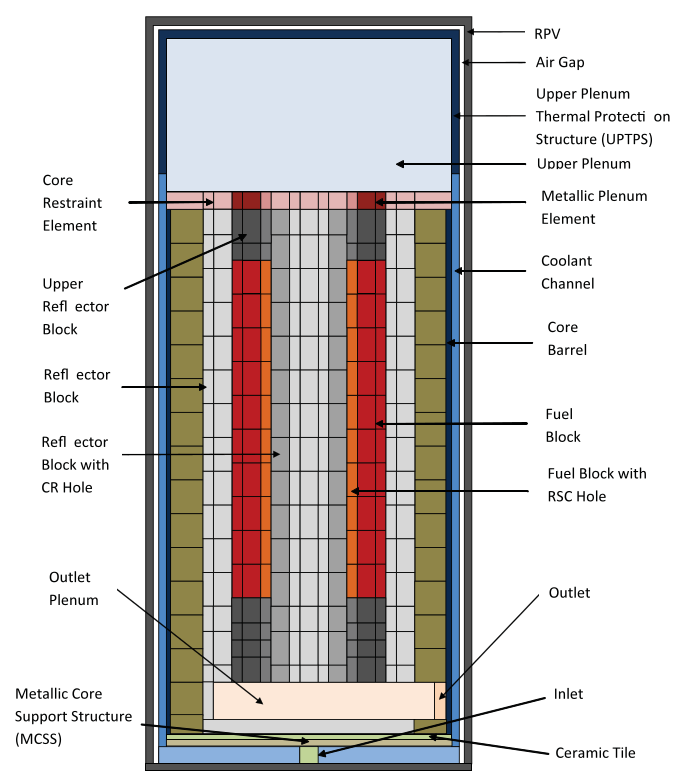
\includegraphics[width=0.45\textwidth]{figures/axial-layout.png}
    }
    \hfill
    \caption{MHTGR-350 reactor layout.}
    \label{fig:layout}
\end{figure}

\begin{table}[htbp!]
  \centering
  \caption{MHTGR-350 Characteristics \cite{oecd_nea_benchmark_2017}.}
  \begin{tabular}{lc}
  \toprule
  Characteristics                   & Value               \\ \midrule
  Installed Thermal Capacity        & 350 MWth            \\
  Installed Electric Capacity       & 165 MWe             \\
  Core inlet/outlet Temperature     & 259/687 $^{\circ}$C    \\
  Power Density                     & 5.9 MW$ \cdot m^{-3}$  \\
  Reactor Vessel Outside diam.      & 6.8 m               \\
  Reactor Vessel Height             & 22 m                \\
  Active core radius                & 2.97 m              \\
  Active core height                & 7.93 m              \\
  Top reflector height              & 1.20 m              \\
  Bottom reflector height           & 1.60 m              \\
  Number of fuel columns            & 66                  \\
  Number of inner reflector columns & 19                  \\
  Number of outer reflector columns & 78                  \\
  \bottomrule
  \end{tabular}
  \label{tab:maincharac}
\end{table}

The core has two types of fuel elements: a standard element and a reserve shutdown element that contains a channel for Reserve Shutdown Control, Figure \ref{fig:fuelassembly}.
Table \ref{tab:element-characteristics} specifies the details of the MHTGR-350 fuel elements.
Twelve columns in the core contain Reserve Shutdown Control channels for borated graphite pellets.
Hoppers above the core house the pellets, and if the control rods become inoperable, the pellets drop into the channels \cite{oecd_nea_benchmark_2017}.

\begin{figure}[htbp!]
  \centering
    \subfloat[Standard fuel assembly. Image reproduced form \cite{tak_numerical_2008}.]{
        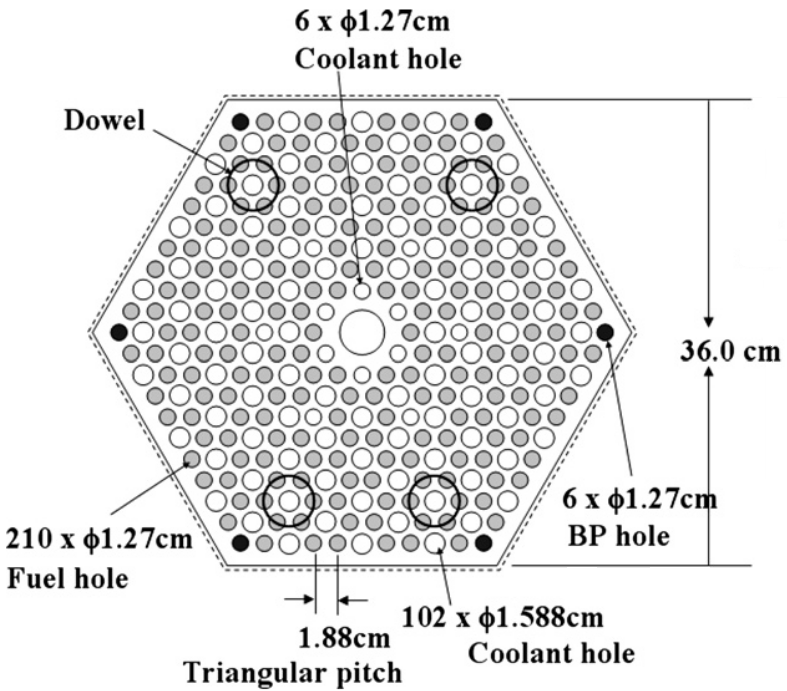
\includegraphics[width=0.45\textwidth]{figures/fuel-assembly}
    }
    \subfloat[RSC fuel assembly. Image reproduced form \cite{tak_practical_2012}.]{
        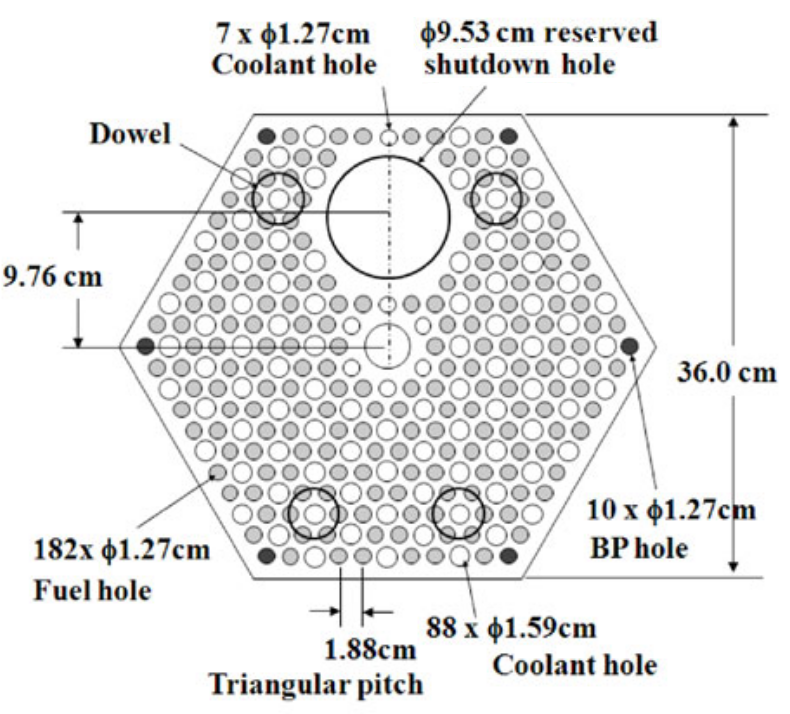
\includegraphics[width=0.45\textwidth]{figures/fuel-assembly-rsc}
    }
  \hfill
    \caption{MHTGR-350 fuel assembly layout.}
  \label{fig:fuelassembly}
\end{figure}

\begin{table}[htbp!]
\centering
      \caption{MHTGR350 fuel element characteristics \cite{oecd_nea_benchmark_2017}.}
      \label{tab:element-characteristics}
    \begin{tabular}{@{}l S[table-format=2.2] c}
    \toprule
    \multicolumn{1}{c}{Shared characteristics} & \multicolumn{1}{c@{}}{Value} & \multicolumn{1}{c@{}}{Units} \\
    \midrule
  Block pitch (flat-to-flat)       & 36      & cm       \\
  Fuel length                      & 79.3    & cm       \\
  Fuel handling diameter           & 3.5     & cm       \\
  Fuel handling length             & 26.4    & cm       \\
  RSC hole diameter                & 9.525   & cm       \\
  RSC center to assembly center    & 9.756   & cm       \\
  Fuel/coolant pitch               & 1.879   & cm       \\
  Fuel hole radius                 & 0.635   & cm       \\
  Compacts per fuel hole           & \multicolumn{1}{c@{}}{15}    & -        \\
  Large coolant hole radius        & 0.794   & cm       \\
  Small coolant hole radius        & 0.635   & cm       \\
  Burnable posion hole radius      & 0.635   & cm       \\
  Block graphite density           & 1.85    & g $\cdot cm^{-3}$ \\
  \midrule

      \multicolumn{1}{c}{Standard element} &  &  \\

  \midrule
  Number of large coolant holes    & \multicolumn{1}{c@{}}{120}   & -        \\
  Number of small coolant holes    & \multicolumn{1}{c@{}}{6}     & -        \\
  Number of fuel holes             & \multicolumn{1}{c@{}}{210}   & -        \\
  \midrule

      \multicolumn{1}{c}{RSC element} &  &  \\

  \midrule
  Number of large coolant holes    & \multicolumn{1}{c@{}}{88}    & -        \\
  Number of small coolant holes    & \multicolumn{1}{c@{}}{7}     & -        \\
  Number of fuel holes             & \multicolumn{1}{c@{}}{186}   & -        \\
    \bottomrule
    \end{tabular}
\end{table}

% Fuel assemblys and triso particles
The fuel elements contain blind holes for fuel compacts and full-length channels for helium coolant flow.
Table \ref{tab:compact} specifies the details of the TRISO particle and fuel compact designs of the \gls{MHTGR}-350.

\begin{table}[htbp!]
\centering
    \caption{TRISO and fuel compact characteristics \cite{oecd_nea_benchmark_2017}.}
    \label{tab:compact}
    \begin{tabular}{@{}l S[table-format=2.3] c}
    \toprule
    \multicolumn{1}{c}{Characteristic} & \multicolumn{1}{c@{}}{Value} & \multicolumn{1}{c@{}}{Units} \\
    \midrule
  Fuel                             & UC$_{0.5}$O$_{1.5}$   & -        \\
  Enrichment (average)             & 15.5                  & wt\%     \\
  Packing fraction (average)       & 0.35                  & -        \\
  Kernel radius                    & 0.02125               & cm       \\
  Buffer radius                    & 0.03125               & cm       \\
  IPyC radius                      & 0.03475               & cm       \\
  SiC radius                       & 0.03825               & cm       \\
  OPyC radius                      & 0.04225               & cm       \\
  Compact radius                   & 0.6225                & cm       \\
  Compact gap radius               & 0.6350                & cm       \\
  Compact length                   & 4.9280                & cm       \\
  Kernel density                   & 10.50                 & g $\cdot cm^{-3}$ \\
  Buffer density                   & 1.00                  & g $\cdot cm^{-3}$ \\
  IPyC density                     & 1.90                  & g $\cdot cm^{-3}$ \\
  SiC density                      & 3.20                  & g $\cdot cm^{-3}$ \\
  OPyC density                     & 1.90                  & g $\cdot cm^{-3}$ \\
  Compact matrix density           & 1.74                  & g $\cdot cm^{-3}$ \\
    \bottomrule
    \end{tabular}
\end{table}

% Reactivity control
A combination of lumped burnable poison and control rods manages the core reactivity.
The lumped burnable poison consists of \gls{B4C} granules dispersed in graphite compacts.
The current design uses six lumped burnable poison rods per element.
Table \ref{tab:LBP} displays the characteristics of the lumped burnable poison compacts.
The reactor has 30 control rods.
Six are for reactor start-up and are in the inner reflector, while the remaining 24 are operating control rods and manage the reactivity during power operation and reactor trips.

\begin{table}[htbp!]
\centering
    \caption{Burnable poison compact characteristics \cite{oecd_nea_benchmark_2017}.}
    \label{tab:LBP}
    \begin{tabular}{@{}l S[table-format=1.4] c}
    \toprule
    \multicolumn{1}{c}{Characteristic} & \multicolumn{1}{c@{}}{Value} & \multicolumn{1}{c@{}}{Units} \\
    \midrule
  Absorber                         & B$_{4}$C              & -         \\
  Packing fraction                 & 0.109                 & -         \\
  Kernel radius                    & 0.0100                & cm        \\
  Buffer radius                    & 0.0118                & cm        \\
  PyC radius                       & 0.0141                & cm        \\
  Compact radius                   & 0.5715                & cm        \\
  Compact gap radius               & 0.6350                & cm        \\
  Rod length                       & 72.187                & cm        \\
  Kernel density                   & 2.47                  & g $\cdot cm^{-3}$ \\
  Buffer density                   & 1.00                  & g $\cdot cm^{-3}$ \\
  PyC density                      & 1.87                  & g $\cdot cm^{-3}$ \\
  Compact matrix density           & 0.94                  & g $\cdot cm^{-3}$ \\
    \bottomrule
    \end{tabular}
\end{table}


\section{Organization of the Simulations}

This thesis separates the description of Moltres simulations into Chapters \ref{ch:neutronics} and \ref{ch:thermalfluids}.
Chapter \ref{ch:neutronics} focuses on stand-alone neutronics simulations in which Moltres solves equations \ref{eq:diffusion-eig} and \ref{eq:heatsource2} to calculate the multiplication factor, the neutron flux, and the radial power distribution.
Chapter \ref{ch:neutronics} discusses two main validation exercises.
The first exercise compares a Serpent and Moltres model of the MHTGR-350.
Serpent obtains the multiplication factor, the neutron flux distribution, and the radial power distribution in the reactor core.
Serpent also generates the group constants of the MHTGR-350 that serve as an input for Moltres simulations.
The second exercise follows Phase I Exercise 1 of the OECD/NEA MHTGR-350 Benchmark using Moltres.
The benchmark exercise specifies the group constants that Moltres uses in the simulations.

Chapter \ref{ch:thermalfluids} focuses on stand-alone thermal-fluids and coupled neutronics/thermal-fluid simulations.
Chapter \ref{ch:thermalfluids} discusses several exercises to validate the thermal-fluids model, in which Moltres solves equations \ref{eq:tempsolid}-\ref{eq:film-conduc} to calculate the solid and coolant temperatures.
The first validation exercises study the accuracy of the thermal-fluids model in several configurations, including an equivalent cylindrical model of a unit cell, a three-dimensional unit cell, and a three-dimensional fuel column.
The next exercise follows Phase I Exercise 2 of the OECD/NEA MHTGR-350 Benchmark using Moltres.
Chapter \ref{ch:thermalfluids} also describes a coupling exercise that follows Phase I Exercise 3 of the OECD/NEA MHTGR-350 Benchmark using Moltres.
